\documentclass[12pt,a4paper]{article}

\usepackage[UTF8]{ctex}
\usepackage[scale=0.8]{geometry}
\usepackage{latexsym,amsmath,amsfonts,amssymb,mathrsfs,bm}
\usepackage{abstract,appendix,titlesec,titletoc}
\usepackage{diagbox,booktabs,longtable,tabularx}
\usepackage[amsmath,thmmarks,hyperref]{ntheorem}
\usepackage{fancyhdr,indentfirst}
\usepackage[colorlinks=ture]{hyperref}
\usepackage{makeidx,cleveref}
\usepackage[sort&compress, numbers]{natbib}
\usepackage{graphicx,epsfig,subfig}
\usepackage{algorithm,algorithmicx,algpseudocode}
\usepackage{xcolor}

\linespread{1.3}
\setlength{\parskip}{0.5\baselineskip}

\theoremstyle{plain}
\newtheorem{definition}{定义}
\newtheorem{example}{例}
\newtheorem{theorem}{定理}
\newtheorem{lemma}{引理}
\newtheorem{corollary}{推论}
\newtheorem{remark}{注}
\newtheorem{proposition}{性质}

\newcommand{\Rnum}{\mathbb{R}}
\newcommand{\Cnum}{\mathbb{C}}
\newcommand{\Znum}{\mathbb{Z}}
\newcommand{\Nnum}{\mathbb{N}}
\newcommand{\Prob}{\mathbb{P}}
\newcommand{\bx}{\mathbf{x}}
\newcommand{\by}{\mathbf{y}}
\newcommand{\bn}{\mathbf{n}}

\title{任意网格上的边自由度有限体积格式}
\author{刘子旗~\&~苗帅}
\date{\today}

\begin{document}

\maketitle

一般在扭曲网格上的有限体积格式,未知量都定义在单元中心和网格节点上。这里我们构造一族未知量定义在网格边上的有限体积格式。对于边自由度有限体积的框架下,我们证明了收敛性。

\section*{问题介绍}

区域$\Omega$是二维多边形区域。我们要在区域上求解稳态扩散问题
\begin{equation*}
\begin{split}
- \nabla \cdot (\kappa \, \nabla u) = f & \quad x \in \Omega \\
u(x) = u_0 & \quad x \in \partial \Omega
\end{split}
\end{equation*}
其中$u(x)$是未知函数,$\kappa(x)$是$2 \times 2$对称正定的矩阵,表示张量型的扩散系数。

我们希望在任意多边形网格上求解方程。多边形网格由单元,节点和边组成。如图\ref{f1},边$AB$是单元$K$和单元$L$之间的边,它的中点为$E$。我们把单元中心和节点连接起来(虚线),使得每条边都被包围在一个四边形内。虚线所组成的网格叫做对偶网格,每条边对应的四边形叫做边控制体。

\begin{figure}[h]
\centering
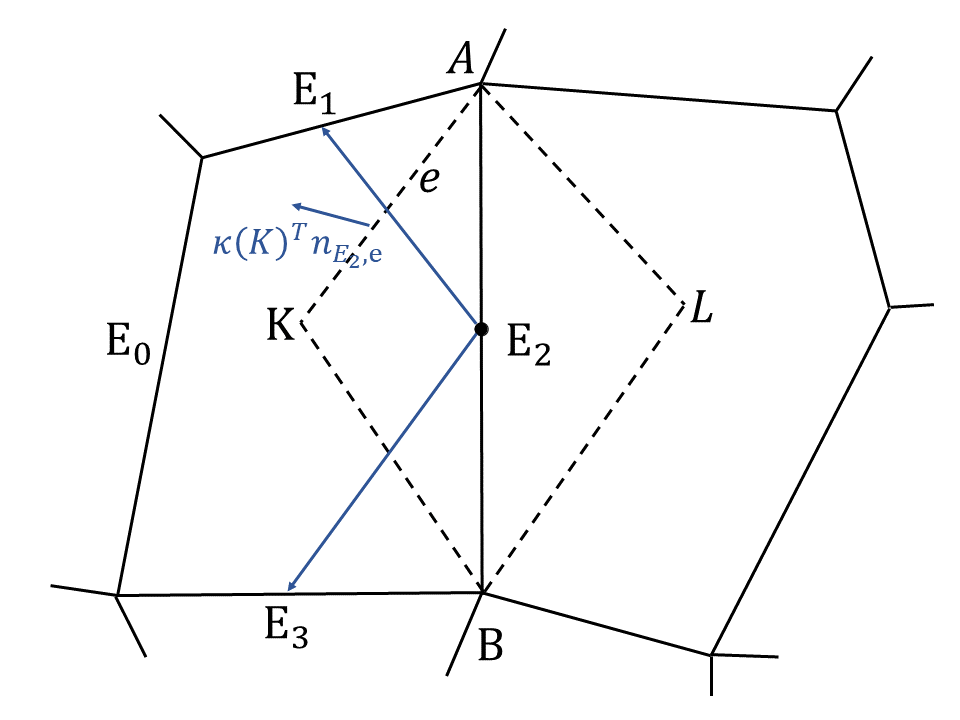
\includegraphics[width=0.5\linewidth]{stencil.png}
\caption{数值格式的网格和模板}
\label{f1}
\end{figure}

\section*{格式构造}

在图中虚线围成的四边形$AKBL$中,对方程两边积分,用散度定理得到
\begin{equation*}
- \int_{AKBL} \nabla \cdot (\kappa(x) \, \nabla u(x)) \ dx = - \sum_{\sigma = KA, AL, LB, BK} \int_{\sigma} (\kappa(x) \, \nabla u(x)) \cdot n_{E, \sigma} \ dx = \int_{K} f(x) \ dx
\end{equation*}
其中$n_{E, \sigma}$表示虚线对应的法方向,也就是四边形的外法方向。

我们假设扩散系数在每个单元上近似为常数。$\kappa(x) = \kappa(K) + \mathcal{O}(h)$。
在虚线网格边上的流量可以表示为
\begin{equation*}
F_{E, \sigma} = - \int_{\sigma} (\kappa(x) \, \nabla u(x)) \cdot n_{E, \sigma} \ dx = |\sigma| \,  \nabla u(x) \cdot \kappa(K)^T \, n_{E, \sigma} + \mathcal{O}(h^2)
\end{equation*}

下面我们给出两种通过边自由度近似流量的方法。 

\subsection*{边自由度格式}

如图\ref{f1},在单元$K$中,边$E_0,E_1,E_2,E_3$顺时针排列。考虑$E_2$对应的边控制体,在计算对偶网格边$\sigma$上的流量时,我们把联合法向量$\kappa(K)^T \, n_{E_2, \sigma_2}$分解成$\overrightarrow{E_2 E_1}, \overrightarrow{E_2 E_3}$的组合,即
\begin{align*}
|\sigma| \kappa(K)^T n_{E_2, \sigma_2} = \alpha_1 \, \overrightarrow{E_2 E_1} + \alpha_2 \, \overrightarrow{E_2 E_3}
\end{align*}
根据方向导数的性质
\begin{align*}
\nabla u \cdot \overrightarrow{E_2 E_1} = u(E_1) - u(E_2) + \mathcal{O}(h)
\end{align*}
得到流量表示为
\begin{align*}
F_{E_2, \sigma_2} = (\alpha_{1} \, (u(E_2) - u(E_1)) + \alpha_{2} \, (u(E_2) - u(E_3))) + \mathcal{O}(h^2)
\end{align*}
这样我们就给出了流量的表达式。

同理,在相邻的边控制体上,我们也可以得到另一侧的流量$F_{E_1, \sigma}$。既然两个流量都是二阶的,考虑到流守恒的要求,我们可以把两个流平均起来,就得到了最终的流量。(此处要注意符号,$E_1$和$E_2$上计算的流量都是以向外为正方向)
\begin{align*}
F_{\sigma} = \frac12 (F_{E_1, \sigma_2} - F_{E_2, \sigma_2})
\end{align*}

\subsection*{边自由度格式的一般框架}

对于原网格中的单元$K$,单元中包含$n$条对偶网格边$\sigma_1,\cdots,\sigma_n$,这些网格边上的流量用$\mathbf{F}_K = (F_1,\cdots,F_n)^T$表示。构造边自由度格式,就是要用定义在网格边上的未知量$\delta \mathbf{U}_K = (u_{E_n}-u_{E_1},\cdots,u_{E_{n-1}}-u_{E_{n}})^T$,表示出边上的流量。

对于线性格式,流量通过边未知量线性表示
\begin{align*}
\mathbf{F}_K = A_K \, \delta \mathbf{U}_K
\end{align*}



\section*{强制性证明}
















\section*{实验结果}

\subsection*{实验1}

求解稳态扩散方程,精确解和扩散系数选为
\begin{align*}
u = \sin((x-1)(y-1)) - (x-1)^3 (y-1)^2 \qquad
a = \left[
\begin{matrix}
1.5 & 0.5 \\
0.5 & 1.5 \\
\end{matrix}
\right]
\end{align*}
网格为随机多边形网格,使用的网格和结果如图。

\begin{figure}[H]
\centering
\subfloat[多边形网格]{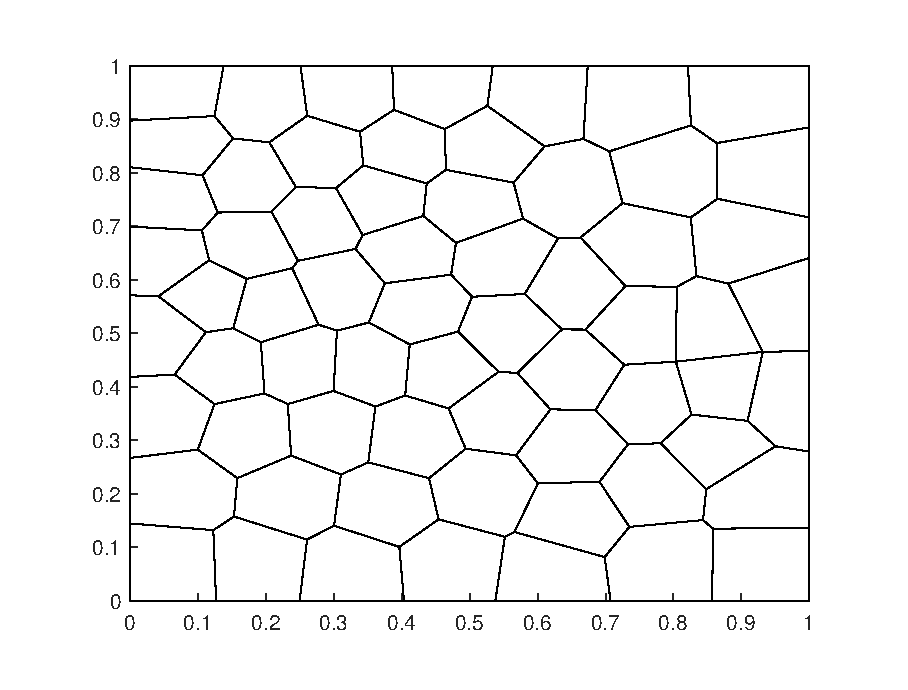
\includegraphics[width=0.3\linewidth]{mesh1}}
\subfloat[数值解$u_h$]{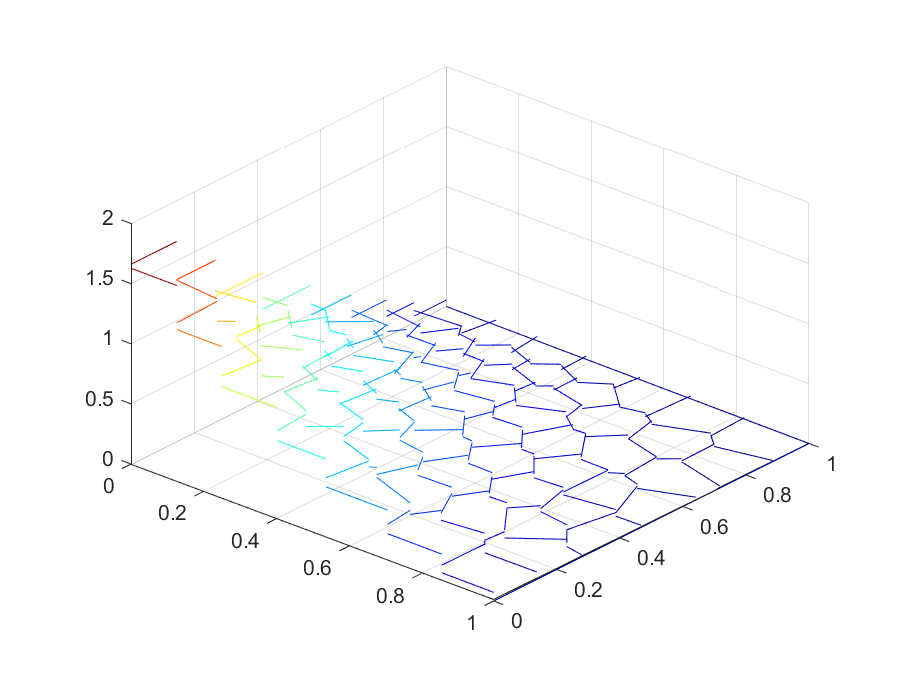
\includegraphics[width=0.3\linewidth]{u1}}
\subfloat[误差$u - u_h$]{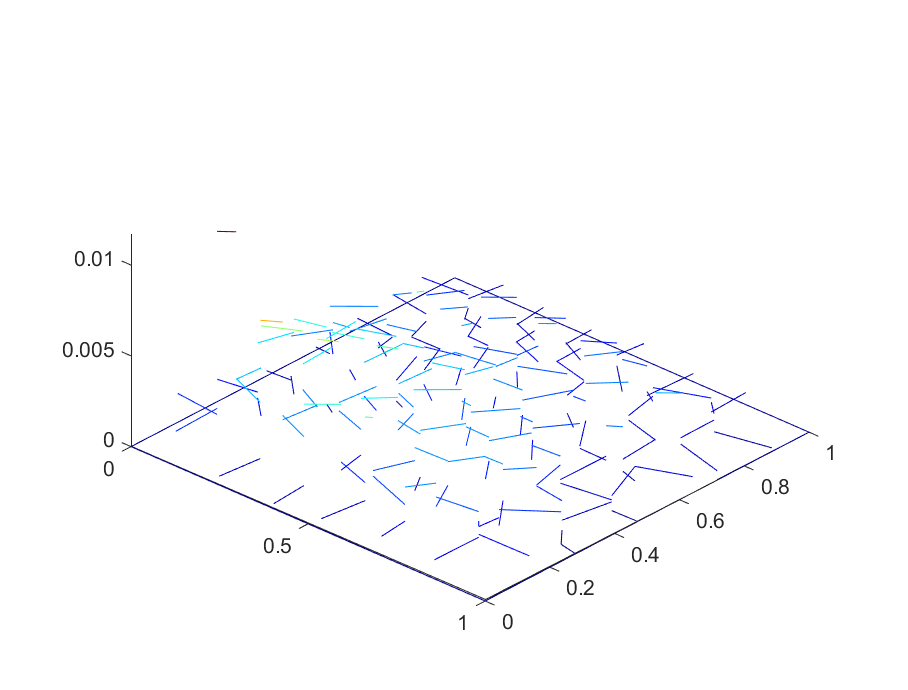
\includegraphics[width=0.3\linewidth]{e1}}
\caption{实验结果1}
\end{figure}

在这样的网格上,误差已经达到了$10^{-2}$。

\subsection*{实验2}

精确解和扩散系数选为
\begin{align*}
u = 16 \, x \, y \, (1-x) \, (1-y) \qquad
a = \left[
\begin{matrix}
1.5 & 0.5 \\
0.5 & 1.5 \\
\end{matrix}
\right]
\end{align*}
使用的网格如图。对网格不断加密,得到收敛阶如下表
\begin{figure}[H]
\centering
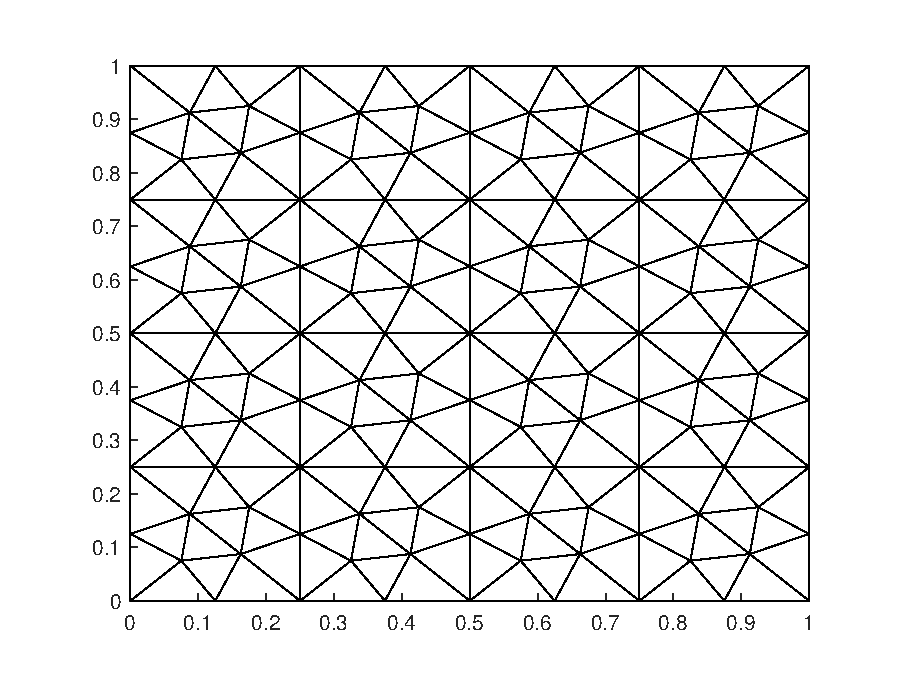
\includegraphics[width=0.4\linewidth]{mesh2}
\caption{实验2网格}
\end{figure}

\begin{table}
\centering
\begin{tabular}{ccc|ccc}
\multicolumn{3}{c}{九点有限体积格式}  & \multicolumn{3}{c}{边中点有限体积格式} \\
\hline
DOF & $\|u - u_h\|_{\infty}$ & order & DOF & $\|u - u_h\|_{\infty}$ & order \\
\hline
56 & 4.32e-02 & * & 92 & 5.43e-02 & * \\
224 & 1.08e-02 & 1.99381 & 352 & 1.77e-02 & 1.67478 \\
896 & 2.72e-03 & 1.99582 & 1376 & 4.96e-03 & 1.86234 \\
3584 & 6.81e-04 & 1.99781 & 5440 & 1.31e-03 & 1.93628 \\
14336 & 1.70e-04 & 1.99893 & 21632 & 3.37e-04 & 1.9693 \\
\hline
\end{tabular}
\end{table}

边中点有限体积格式可以达到二阶收敛,而且在某些特殊的网格上,它比九点格式更有优势。

%\bibliographystyle{plain}
%\bibliography{FVM}

\end{document}